\documentclass[border=8pt]{standalone}
\usepackage{tikz}
\usetikzlibrary{arrows.meta,positioning,calc}
\begin{document}
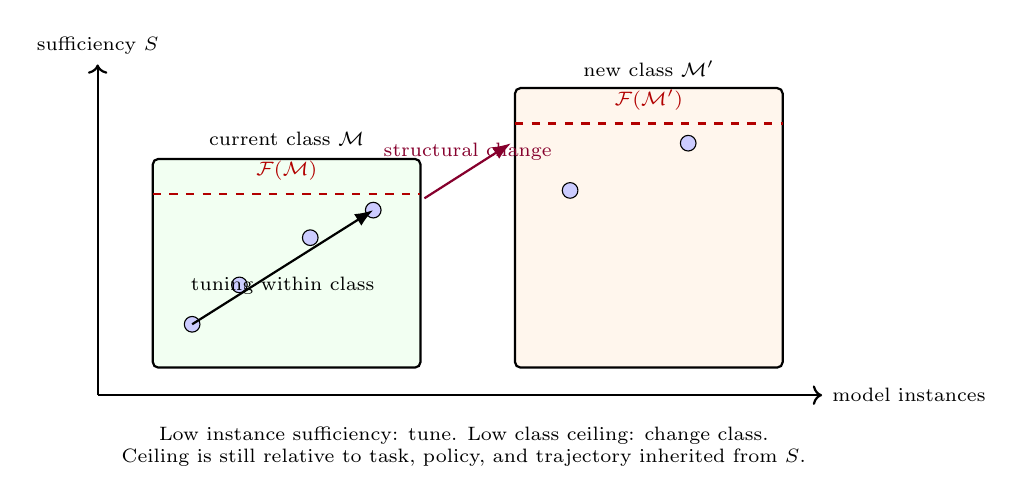
\begin{tikzpicture}[
  point/.style={circle, draw, fill=blue!20, inner sep=2pt},
  arr/.style={-Latex, thick},
  note/.style={align=center, font=\scriptsize}
]

\draw[->, thick] (0,0) -- (0,4.2) node[above, note] {sufficiency $S$};
\draw[->, thick] (0,0) -- (9.2,0) node[right, note] {model instances};

\draw[thick, rounded corners=2pt, fill=green!5] (0.7,0.35) rectangle (4.1,3.0);
\node[note] at (2.4,3.25) {current class $\mathcal M$};
\draw[red!70!black, thick, dashed] (0.7,2.55) -- (4.1,2.55);
\node[note, red!70!black] at (2.4,2.85) {$\mathcal F(\mathcal M)$};

\node[point] at (1.2,0.9) {};
\node[point] at (1.8,1.4) {};
\node[point] at (2.7,2.0) {};
\node[point] at (3.5,2.35) {};
\draw[arr] (1.2,0.9) -- node[below, note] {tuning within class} (3.5,2.35);

\draw[thick, rounded corners=2pt, fill=orange!7] (5.3,0.35) rectangle (8.7,3.9);
\node[note] at (7.0,4.15) {new class $\mathcal M'$};
\draw[red!70!black, thick, dashed] (5.3,3.45) -- (8.7,3.45);
\node[note, red!70!black] at (7.0,3.75) {$\mathcal F(\mathcal M')$};
\node[point] at (6.0,2.6) {};
\node[point] at (7.5,3.2) {};

\draw[arr, thick, purple!70!black] (4.15,2.5) -- node[above, note] {structural change} (5.25,3.2);

\node[note] at (4.65,-0.65) {Low instance sufficiency: tune. Low class ceiling: change class.\\Ceiling is still relative to task, policy, and trajectory inherited from $S$.};

\end{tikzpicture}
\end{document}
